\documentclass[a4paper,9pt,onecolumn]{ltjsarticle} % ← lualatex ではなく ltjsarticle
\usepackage[ipaex]{luatexja-preset}  % 日本語フォントの手当て(IPAex)
\usepackage{ifthen}
\usepackage{algorithm}
\usepackage{algpseudocode}
\usepackage{amsmath}
\usepackage{graphicx}
\usepackage{here}
\usepackage{algpseudocode}
\usepackage{titlesec}

\makeatletter
\renewcommand{\maketitle}{%
\ifthenelse{\equal{\course}{bachelor}}{%
  \begin{titlepage}
    \vspace*{10mm}
    \begin{center}
      {\huge\@gyear 年度\hspace{5mm}\@thesis\par}
      \vfill
      {\huge\bfseries\@title\par}
      \vfill
      \vspace{10mm}
      {\Large\@date\par}
      \vspace{20mm}
      {\Large\@department\@departmentsfx\par}
      {\Large (学生番号: \@studentid)\par}
      \vspace{5mm}
      {\LARGE\@author\par}
      \vspace{55mm}
      {\Large 和歌山大学\@faculty}
      \vspace{10mm}
    \end{center}
  \end{titlepage}}{}%
\ifthenelse{\equal{\course}{master}}{%
  \begin{titlepage}
    \begin{center}
      \vspace*{8mm}
      {\Large\@gyear 年度\hspace{5mm}\@thesis\par}
      \vfill
      {\huge\bfseries\@title\par}
      \vfill
      {\Large \@date\par}
      \vspace{40mm}
      {\Large 和歌山大学\@faculty\par}
      \vspace{27mm}
      {\Large 学生番号: \@studentid\par}
      {\LARGE \@author\par}
      \vspace*{28mm}
    \end{center}
  \end{titlepage}%
  \begin{titlepage}
    \begin{center}
      \vspace*{8mm}
      {\huge\@etitle\par}
      \vspace{12mm}
      {\Large by\par}
      \vspace{9mm}
      {\huge\@eauthor\par}
      \vspace{27mm}
      {\LARGE\@ethesis\par}
      \vfill
      {\Large \@efaculty\par}
      \vspace{4mm}
      {\Large Wakayama University\par}
      \vspace{23mm}
      {\Large \@edate\par}
      \vspace*{14mm}
    \end{center}
  \end{titlepage}}{}%
}

%% 概要
\def\abstract{\newpage\pagenumbering{roman}\section*{概 要}}
\def\endabstract{}
%% 目次
\def\tableofcontents{
  \newpage
  \section*{目 次\@mkboth{目 次}{目 次}}
  \@starttoc{toc}}
%% 図目次
\def\listoffigures{%
  \newpage
  \section*{図 目 次\@mkboth{図 目 次}{図 目 次}}
  \@starttoc{lof}}
%% 表目次
\def\listoftables{%
  \newpage
  \section*{表 目 次\@mkboth{表 目 次}{表 目 次}}
  \@starttoc{lot}}
%% 謝辞
\def\acknowledgements{\newpage\section*{謝 辞}}
\def\endacknowledgements{}
%% 参考文献
\def\thebibliography#1{%
  \newpage
  \section*{参 考 文 献\@mkboth{参 考 文 献}{参 考 文 献}}
  \list{[\arabic{enumi}]}
    {\settowidth{\labelwidth}{[#1]}
     \leftmargin=\labelwidth
     \advance\leftmargin by \labelsep
     \usecounter{enumi}}
  \def\newblock{\hskip .11em plus .33em minus .07em}
  \sloppy
  \clubpenalty=4000 \widowpenalty=4000
  \sfcode`\.=1000\relax}
\let\endthebibliography=\endlist
\makeatother

\makeatletter
\def\course{bachelor}
\def\@gyear{2025}
\def\@thesis{卒業論文}
\def\@title{分散型IoTデータ管理に向けたIPFSを用いたDID発行・検証システム}
\def\@date{2026年2月10日}
\def\@department{システム工学部}
\def\@departmentsfx{システム工学科}
\def\@studentid{60276128}
\def\@author{竹内 結哉}
\def\@faculty{システム工学部}
\makeatother

\newcommand{\sectionbreak}{\clearpage}

\begin{document}
\maketitle
\tableofcontents

\section{はじめに}
近年,IoT機器の爆発的な増加に伴い,生成されるデータ量は急激に増加している.
さらに,IoTは家庭や産業,医療,農業など多様な分野で活用されるようになり,生成されるデータの種類や粒度も一層多様化している.

また,従来の中央集権型によるIoTデータ管理には主に次の3つの課題が存在する.

第一に,スケーラビリティの問題である.
IoTデバイスの急増により,そのデータを保存する中央サーバーへの負荷が指数関数的に増大し,処理能力の限界に達する可能性がある.

第二に,セキュリティ上の問題である.中央サーバーは単一障害点となりやすく,攻撃対象として脆弱である.

第三に,プライバシー保護の問題である.個人情報を含むIoTデータが集中することで,情報漏洩時の被害が甚大化するリスクがある.

これらの課題を解決するために,本研究ではユーザ主権型IDに基づいた分散型データ管理システムの実現を目指す.
本研究における提案システムは,以下の三点を重視して設計されている.

\begin{enumerate}
\item データの分散管理:中央集権型管理から脱却し,分散型ファイルシステムであるInterPlanetary File System(以下IPFS)を用いることで,
      単一障害点を排除しシステムの堅牢性を向上させる.
\item ユーザの真正性確保:分散管理環境におけるなりすまし防止のため,分散型識別子であるDecentralized identifier(以下DID)を活用し,
      データ所有者の身元を保証する.
\item データの信頼性と改ざん防止:ブロックチェーンを活用し,データが改ざんされていないことを検証可能とする.
\end{enumerate}
以上の要素を組み合わせることで,IoTデータに対する分散型かつ信頼可能な管理基盤を構築することを目指す.

\section{関連研究}
IoTデータ管理に関する研究では,デバイス数の増加に伴うスケーラビリティの確保や,
データの完全性・真正性をいかに保証するかが重要な課題として指摘されてきた.
特に,従来の中央集権型アーキテクチャに基づくデータ管理では,
管理主体への依存や単一障害点の存在により,
可用性やセキュリティ,プライバシーの観点でリスクが生じやすいことが問題とされている.
これらの課題を背景として,近年ではブロックチェーンや分散型ストレージを活用した,
中央集権的管理に依存しないIoTデータ管理手法が数多く提案されている.

Aliら\cite{cite1}は,中央集権的なIoTデータ管理における管理主体への依存やスケーラビリティの問題を指摘し,
ブロックチェーンとIPFSを組み合わせたモジュラー・コンソーシアム・アーキテクチャを提案している.
この手法では,IoTデータ本体をIPFSに保存し,ブロックチェーンにはそのハッシュ値のみを記録することで,
データ管理の分散化と改ざん耐性を両立している.
また,IoTデバイス群ごとにサイドチェーンを構成する設計により,
単一のブロックチェーンに処理が集中することを回避し,分散的なIoTデータ管理におけるスケーラビリティ確保の重要性を示している.

Krejciら\cite{cite2}は,IoTデータ配信におけるデータ完全性とリアルタイム性のトレードオフに着目し,
ブロックチェーンとIPFSを用いたデュアルチャネル型のデータ配信手法を提案している.
提案手法では,リアルタイム性を重視したMQTTによる配信と並行して,IPFS上に保存したデータのハッシュ値をブロックチェーンに記録することで,
後からデータの改ざん検証を可能としている.
評価実験では,ブロックチェーンを用いた完全性検証が高頻度に実行される処理には不向きである一方,
取引時など限定的なタイミングでの検証には有効であることが示されている.

一方,ブロックチェーンをIoTへ適用する際の課題として,
コンセンサス処理に起因する遅延やスループット低下が指摘されている.
Haqueら\cite{cite3}は,Delegated Proof of Stake(DPoS)を用いた軽量コンセンサスとIPFSを組み合わせることで,
多数のIoTデバイスが存在する環境においてもスケーラブルなデータ管理を可能とするフレームワークを提案している.
さらにHaqueら\cite{cite4}は,DPoSに加えてシャーディング技術を導入し,
トランザクション処理の並列化による性能向上を図っており,
IoT環境における処理性能とスケーラビリティ改善の方向性を示している.

これらの流れを医療分野へ適用した研究として,Kebiraら\cite{cite5}は,
IoT,ブロックチェーン,IPFSを統合した分散型ヘルスケアシステム「BlockMedCare」を提案している.
BlockMedCareは,慢性疾患患者の遠隔モニタリングを対象とし,
従来のクライアント/サーバー型医療情報管理における単一障害点やプライバシー侵害のリスクを課題として位置づけている.
提案システムでは,医療データ本体を暗号化した上でIPFSに保存し,
ブロックチェーンにはそのハッシュ値のみを記録することで,スケーラビリティとデータ完全性を両立している.
また,Proof of Authority(PoA)を採用したプライベートブロックチェーンにより,
医療用途に求められる処理性能の向上を実現している.
さらに,プロキシ再暗号化やスマートコントラクトを用いたアクセス制御により,
医療データ共有におけるセキュリティ確保の有効性を示している.

以上の先行研究から,IoTデータ管理においては,データ本体を分散ストレージに保存し,
ブロックチェーンは参照情報や検証情報の管理に限定して用いる設計が,
スケーラビリティと信頼性の両方に有効であることが分かる.
これらの研究は中央集権型管理に内在するリスクを回避する手段として,
ブロックチェーンおよびIPFSを用いた分散型IoTデータ管理の有効性を示すものである.
一方で,データの所有者や提供主体の正当性,すなわち「誰のデータであるか」や「正当な主体が提示しているか」
といった主体に関する検証については,分散環境における主体識別の標準化まで含めて統合的に扱う研究は十分とは言えない.

本研究では,これらの知見を踏まえ,DIDを統合した分散型IoTデータ管理システムの構築を目指す.
DIDにより分散環境における主体識別を明確化し,IoTデータの真正性を第三者が検証可能とすることで,
既存研究では十分に扱われてこなかった主体の正当性検証を含むデータ管理について検討する点に本研究の特徴がある.

\section{準備}
本研究では,分散型データ管理の基盤技術としてIPFS,ブロックチェーンおよびDIDを用いる.
本章では,これらの技術の概要を説明し,さらに本研究で使用した実験環境について述べる.

\subsection{InterPlanetary File System(IPFS)}
IPFSは世界中のコンピュータ(ノード)に分散的にデータを保存するP2P型のファイルシステムである.
IPFSでは中央集権的なサーバーを介さず,データを分散的に管理しており,耐故障性,負荷分散,耐検閲性,改ざん耐性に優れている.
特徴は「コンテンツアドレス方式」である点で,保存されたファイルはその内容を基に計算されるContent Identifier(以下CID)によって参照される.
CIDはファイル内容のハッシュ値であるため,以下の性質を持つ.

\begin{itemize}
  \item 同一内容のファイルは必ず同じCIDとなる.
  \item 1ビットでも内容が変更されれば別のCIDとなる.
  \item CIDから元のデータを推測することはできない.
\end{itemize}
この仕組みにより,ファイルが改ざんされていないかをCIDの比較によって確認できるため,改ざん耐性に優れる.

本研究では,ユーザが保有するIoTデータをIPFSに保存し,得られたCIDをブロックチェーンに記録することで,データの真正性と参照可能性を確保している.

\subsection{ブロックチェーン}
ブロックチェーンは,ネットワーク上の複数のノードが同一のデータを共有し,合意形成に基づいて取引履歴を記録する分散型台帳技術である.
記録されるデータは複数の取引をまとめた「ブロック」に格納され,各ブロックは直前のブロックのハッシュ値を保持することで鎖状に連結される.
この構造により,一部のブロックが改ざんされると以降すべてのブロックの整合性が崩れるため,改ざんは即座に検知される.
ここで重要なのは,ハッシュ値の性質である.
ハッシュ値はデータから一方向的に算出される識別子であり,内容にわずかな変更があっても全く別の値となる.
また,ハッシュ値から元のデータを復元することはできない.
ブロックチェーンではこの性質を利用し,データの完全性を保証している.

本研究では,IoTデータに対応するCIDおよび後述するDIDというユーザの識別子をスマートコントラクト経由でブロックチェーンへ記録することで,
データ登録の証跡を改ざん不能に保持できるようにしている.

さらに,既存研究においても議論されているように,Proof-of-Work(以下PoW)はエネルギー消費が大きく,
リソース制約のあるIoT環境には適さないことが指摘されている\cite{cite2}.
そのため,本研究においてもPoWベースのブロックチェーンは採用せず,より実装や評価に適したEthereum環境を主に使用することとした.

\subsection{Decentralized identifier(DID)}
DIDは特定の中央管理者に依存せずに個人が自分自身で生成・管理できる識別子であり,分散型デジタルアイデンティティの基盤となる技術である.
DIDはそのDIDに紐づく公開メタデータであるDID Documentが存在している必要がある.
DID Documentには識別子の情報やDIDの所有者が使用する公開鍵の情報が含まれており,DIDの正当性や鍵の正しさを検証する場面ではDIDに紐づいたDID Documentを取得して使用される.
DIDからDID Documentを取得するという処理をDID解決と呼ぶ.
DID Documentはブロックチェーンなどの改ざん耐性を持つ基盤に保存されることで,第三者がその内容を検証可能となる.

本研究では,ユーザAおよび発行者が発行したDIDとDID Documentをブロックチェーンに登録し,IoTデータの所有者であることを証明するための基礎情報として利用する.

さらに本研究のシステムでは,発行者がユーザに対してVerifiable Credential(以下VC)と呼ばれる証明書を発行し,
IoTデータが正当なデバイスによって生成されたものであることを保証する仕組みを構築する.
VCの検証時には,DID Documentに記録された公開鍵により署名を確認し,データの真正性を確認することができる.

\section{システム構成}
本研究で提案するシステムは,IoTデータを分散的に管理するために,IPFS,ブロックチェーンおよびDIDを連携させたものである.
本章では,まずシステム全体の流れを示した後,各要素の役割について説明する.

\subsection{システムの概要}
本研究で提案するシステムの全体像を図\ref{fig:system-overview}に示す.
本研究で提案するシステムは,IoTデータを保有するユーザA,データの真正性を確認しVCを発行する発行者,および最終的にVCを検証する検証者により構成される.
図\ref{fig:system-overview}に示すように,ユーザAは自身のIoTデータをIPFSに格納し,その結果として得られるCIDを,
自身の識別子であるDIDとともにブロックチェーンに記録する.
その後,発行者がIoTデータの真正性を保証するVCを発行し,
検証者がブロックチェーン上のDID DocumentとVCを突き合わせることで,ユーザAおよびデータの正当性を検証する.

\begin{figure}[t]
  \centering
  \includegraphics[width=0.9\linewidth]{figures/figure1.png}
  \caption{提案システムの概要図}
  \label{fig:system-overview}
\end{figure}

\subsubsection{データ保有者(ユーザA)}
ユーザAは,自身の識別子としてDIDを保持し,DID Documentをブロックチェーンに格納する.
さらに,保有しているIoTデータをIPFSに格納し,IPFSから返されるCIDを取得する.
ユーザAは,CIDと自身のDIDを組み合わせてブロックチェーンに登録すること,および
後に発行者から取得するVCに自身の秘密鍵で署名することで自身がIoTデータの正当な保有者であることを保証する.

\subsubsection{発行者(企業など)}
発行者とは,ユーザAに対してVCを発行する主体である.
本研究ではユーザAが所持しているIoT機器の製造元企業などを想定している.
発行者はユーザAが保有しているIoTデータが自社製品によって生成されたデータであることを確認し,その真正性を保証するVCをユーザAに発行する.

\subsubsection{検証者}
検証者は,ユーザAとIoTデータを取引する相手,すなわちデータの受領者を想定している.
検証者は,ユーザAから提示されたVCを受け取り,ブロックチェーン上のDID Documentと照合することで,ユーザAが真正なデータ保有者であることや,
IoTデータについて企業が保証していることについて確認することができる.
本研究で提案するシステムにおいては,検証者がVCの正当性を確認した上でデータの取引を実行することを想定している.

\section{システム全体のフロー}
システムの処理は,\textbf{登録フェーズ}と\textbf{検証フェーズ}の2つに大別される.
登録フェーズではDID・IoTデータがブロックチェーンおよびIPFSに記録され,発行者によるVC発行までが行われる.
一方,検証フェーズでは,提示されたVCの署名検証を通じてユーザAが真正なデータ提供者であることを確認し,安全なデータ取引を可能にする.

以下では,両フェーズの詳細な処理について説明する.

\subsection{登録フェーズ}

登録フェーズのフローチャートを図\ref{fig:system_flowchart_regist}に示す.
本フェーズはDIDの生成・登録,IoTデータの保存,CIDの登録,および発行者によるVC発行,ユーザAによるVCへの署名までの流れで構成される.

\subsubsection{DIDの生成とDID Documentの登録}

まず,ユーザAおよび発行者はそれぞれDIDを生成し,それに対応するDID Documentを作成する.
作成したDID Documentはブロックチェーンへ登録される.
DID Documentのブロックチェーンへの登録手順はスマートコントラクト\texttt{registerDIDDocument()}(algorithm~\ref{alg:register_did})で規定される.

本研究では,DIDの制御主体としてEthereumアドレスを用いる設計を採用している.
EthereumアドレスはECDSA(secp256k1)鍵ペアに基づいて生成されるため,
当該アドレスで署名可能であることは対応する秘密鍵を保持していることを意味する.
この対応関係をブロックチェーン上に登録することで,後続処理における署名検証の基盤を構築する.

以下にユーザAが生成したDID Documentの一例を示す.
本DID Documentは最小構成とし,DIDとその制御主体であるEthereumアドレスのみを記載している.

\begin{verbatim}
{
  "id": "did:example:userA",
  "controller": "0x2c854F81C990fDD856fC360f17Dc592366711f08"
}
\end{verbatim}


\subsubsection{IoTデータの保存とCIDの取得}

次に,ユーザAは自身が保有するIoTデータをIPFSに保存する.
この処理により,IoTデータはブロックチェーンとは独立した分散ストレージ上に格納され,
データ本体を直接ブロックチェーンに保存する必要がなくなる.

IPFSへの保存が完了すると,保存されたデータに対応するCIDが取得される.
本研究では,このCIDをIoTデータを一意に識別する参照情報として扱い,
後続の処理においてユーザAのDIDと組み合わせてブロックチェーンへ記録する.

\subsubsection{CIDとDIDのブロックチェーンへの記録}

ユーザAは取得したCIDと自身のDIDをブロックチェーンへ記録する.
CIDとDIDのブロックチェーンへの記録はスマートコントラクト\texttt{registerIoTData()}(algorithm~\ref{alg:register_iot})で規定される.
これにより,「どのDIDがどのIoTデータの所有者であるか」が改ざん耐性を持って記録され,第三者は所有者を検証可能となる.

\subsubsection{発行者によるデータ真正性の確認とVC発行}

発行者は,ブロックチェーン上のDIDとCIDの整合性を確認し,ユーザAが記録したデータが真正であるかを検証する.
正当性が確認された場合,企業はユーザAに対してVCを発行する.
VCには発行者のDIDによる署名が付与され,内容の真正性が保証される.

\subsubsection{ユーザAによるVCへの追加署名}

最後に,ユーザAは自身のDIDに紐づく秘密鍵を用いてVCに追加署名を行う.
これにより,企業とユーザAの双方が署名したVCが完成し,検証フェーズにおいて提示・検証可能な証明情報となる.

\begin{figure}[H]
  \centering
  \includegraphics[height=0.9\textheight, keepaspectratio]{figures/flowchart_regist.png}
  \caption{登録フェーズのフローチャート}
  \label{fig:system_flowchart_regist}
\end{figure}

\subsection{検証フェーズ}

検証フェーズのフローチャートを図\ref{fig:system_flowchart_validate}に示す.
本フェーズでは,ユーザAから提示されたVCに含まれる署名を段階的に検証することにより,
IoTデータが正当なデバイスによって生成されたものであること,およびユーザAが当該データの正当な保有者であることを確認する.

\subsubsection{VCの提示と受領}

ユーザAは,発行者と自身の署名が付与されたVCを検証者に提示する.
検証者は当該VCを受領し,VCに含まれる署名情報および関連付けられたDID Documentを確認することで,
後続の検証処理に備える.

\subsubsection{企業の署名検証}

検証者はまずVCに含まれる発行者の署名を検証する.
署名の公開鍵は,ブロックチェーンへ登録された企業のDID Documentから取得される.
署名が不一致であった場合,VCは不正と判断され処理を終了する.

\subsubsection{ユーザAの署名検証}

企業の署名が正当であった場合,次にユーザAの署名が検証される.
ユーザAの公開鍵は同様にDID Documentから取得され,署名が一致する場合,ユーザAがIoTデータの正当な保有者であることが確認される.
不一致の場合,処理は終了する.

\subsubsection{データの取引の実行}

企業およびユーザAの署名がいずれも正当であれば,検証者はユーザAが真正なデータ提供者であると判断できる.
この確認を基に,検証者はユーザAと安全にデータ取引を実行する.

\begin{figure}[H]
  \centering
  \includegraphics[height=0.9\textheight, keepaspectratio]{figures/flowchart_valid.png}
  \caption{検証フェーズのフローチャート}
  \label{fig:system_flowchart_validate}
\end{figure}

\subsection{スマートコントラクトによる登録処理}

本研究で使用したスマートコントラクトでは,ユーザのDID DocumentおよびIoTデータ(CID)をブロックチェーンに記録するために\texttt{registerDIDDocument}および\texttt{registerIoTData}の2つの関数を提供している.
それぞれの処理内容を擬似コードとして以下に示す.

\begin{algorithm}
\caption{DID Documentの登録処理(registerDIDDocument)}
\label{alg:register_did}
\begin{algorithmic}[1]
\Require DID, DID Document(JSON形式)
\State 呼び出し元アドレスを取得する(これをユーザ識別子として扱う)
\State DID Documentを以下の形式で保存する:
\State \hspace{3mm} \texttt{records[呼び出し元アドレス].append( (DID, DID\_Document) )}
\State DID登録イベントを発行する
\end{algorithmic}
\end{algorithm}

\begin{algorithm}[H]
\caption{IoTデータ(CID)の登録処理(registerIoTData)}
\label{alg:register_iot}
\begin{algorithmic}[1]
\Require DID, CID(IPFSで取得したハッシュ値)
\State 呼び出し元アドレスを取得する
\State IoTデータを以下の形式で保存する:
\State \hspace{3mm} \texttt{IotData[呼び出し元アドレス].append( (DID, CID) )}
\State IoTデータ登録イベントを発行する
\end{algorithmic}
\end{algorithm}

\section{実験と考察}
本章では,本研究で構築したIPFS,ブロックチェーン,DID/VCを用いた分散型データ管理システムについて,機能動作試験および性能評価を通してその有効性を検証する.

\subsection{実験目的}
本研究の実験目的は,大きく2つである.
1つ目は提案システムが問題なく動作することを検証することである.
具体的には,DIDの生成からDID Documentの登録,IoTデータのIPFSへの保存,取得したCIDのブロックチェーンへの記録,発行者によるVCの発行,
および検証者によるVCの検証に至るまでの一連の処理を実装し,それらが想定通り正しく実行されることを確認する.
これにより,IPFS,ブロックチェーン,DID/VCを統合した提案システムが,データとその所有者の正当性を一貫して保証できることを検証する.

2つ目は,提案システムの性能を定量的に評価し,DIDおよびVCを統合したことがシステム全体の性能に与える影響を明らかにすることである.
特に,IPFSおよびブロックチェーンを用いたIoTデータ管理に関する先行研究が多数存在することを踏まえ,これらを基準的な処理として位置づけたうえで,
DIDおよびVCに関連する処理が新たな性能上のボトルネックとなり得るかどうかに着目して評価を行う.

\subsection{実験環境}
本研究における実験は,ノートパソコンおよびRaspberry Piを用いたローカル環境で実施した.
図\ref{fig:experiment_photo}に実際の実験環境の外観を,図\ref{fig:experiment_structure}に実験環境の構成を示す.

Raspberry Piは実際のIoTデバイスの代替として使用し,IoTデータの生成およびノートパソコンへのデータ送信を行う役割を担う.
一方,データ受信後の処理はすべてノートパソコン上で実行しており,
IPFSへのデータ保存,ブロックチェーンへの登録,DIDおよびDID Documentの作成・登録,
並びにVCの発行および検証処理を行っている.

ノートパソコン上で使用したソフトウェアおよび実行環境をいかに示す.

\begin{itemize}
  \item OS:Windows 11 Home
  \item CPU:AMD Ryzen 5 PRO 7530U with Radeon Graphics(2.00Hz)
  \item メモリ:16GB
  \item IPFS:go-ipfs v0.35.0
  \item ブロックチェーン環境:Ganache v7.9.2
  \item Solidity: v0.5.16
  \item Node.js: v18.20.7
  \item Truffle: v5.11.5
  \item Web3.js: v1.10.0
\end{itemize}

\begin{figure}[H]
  \centering
  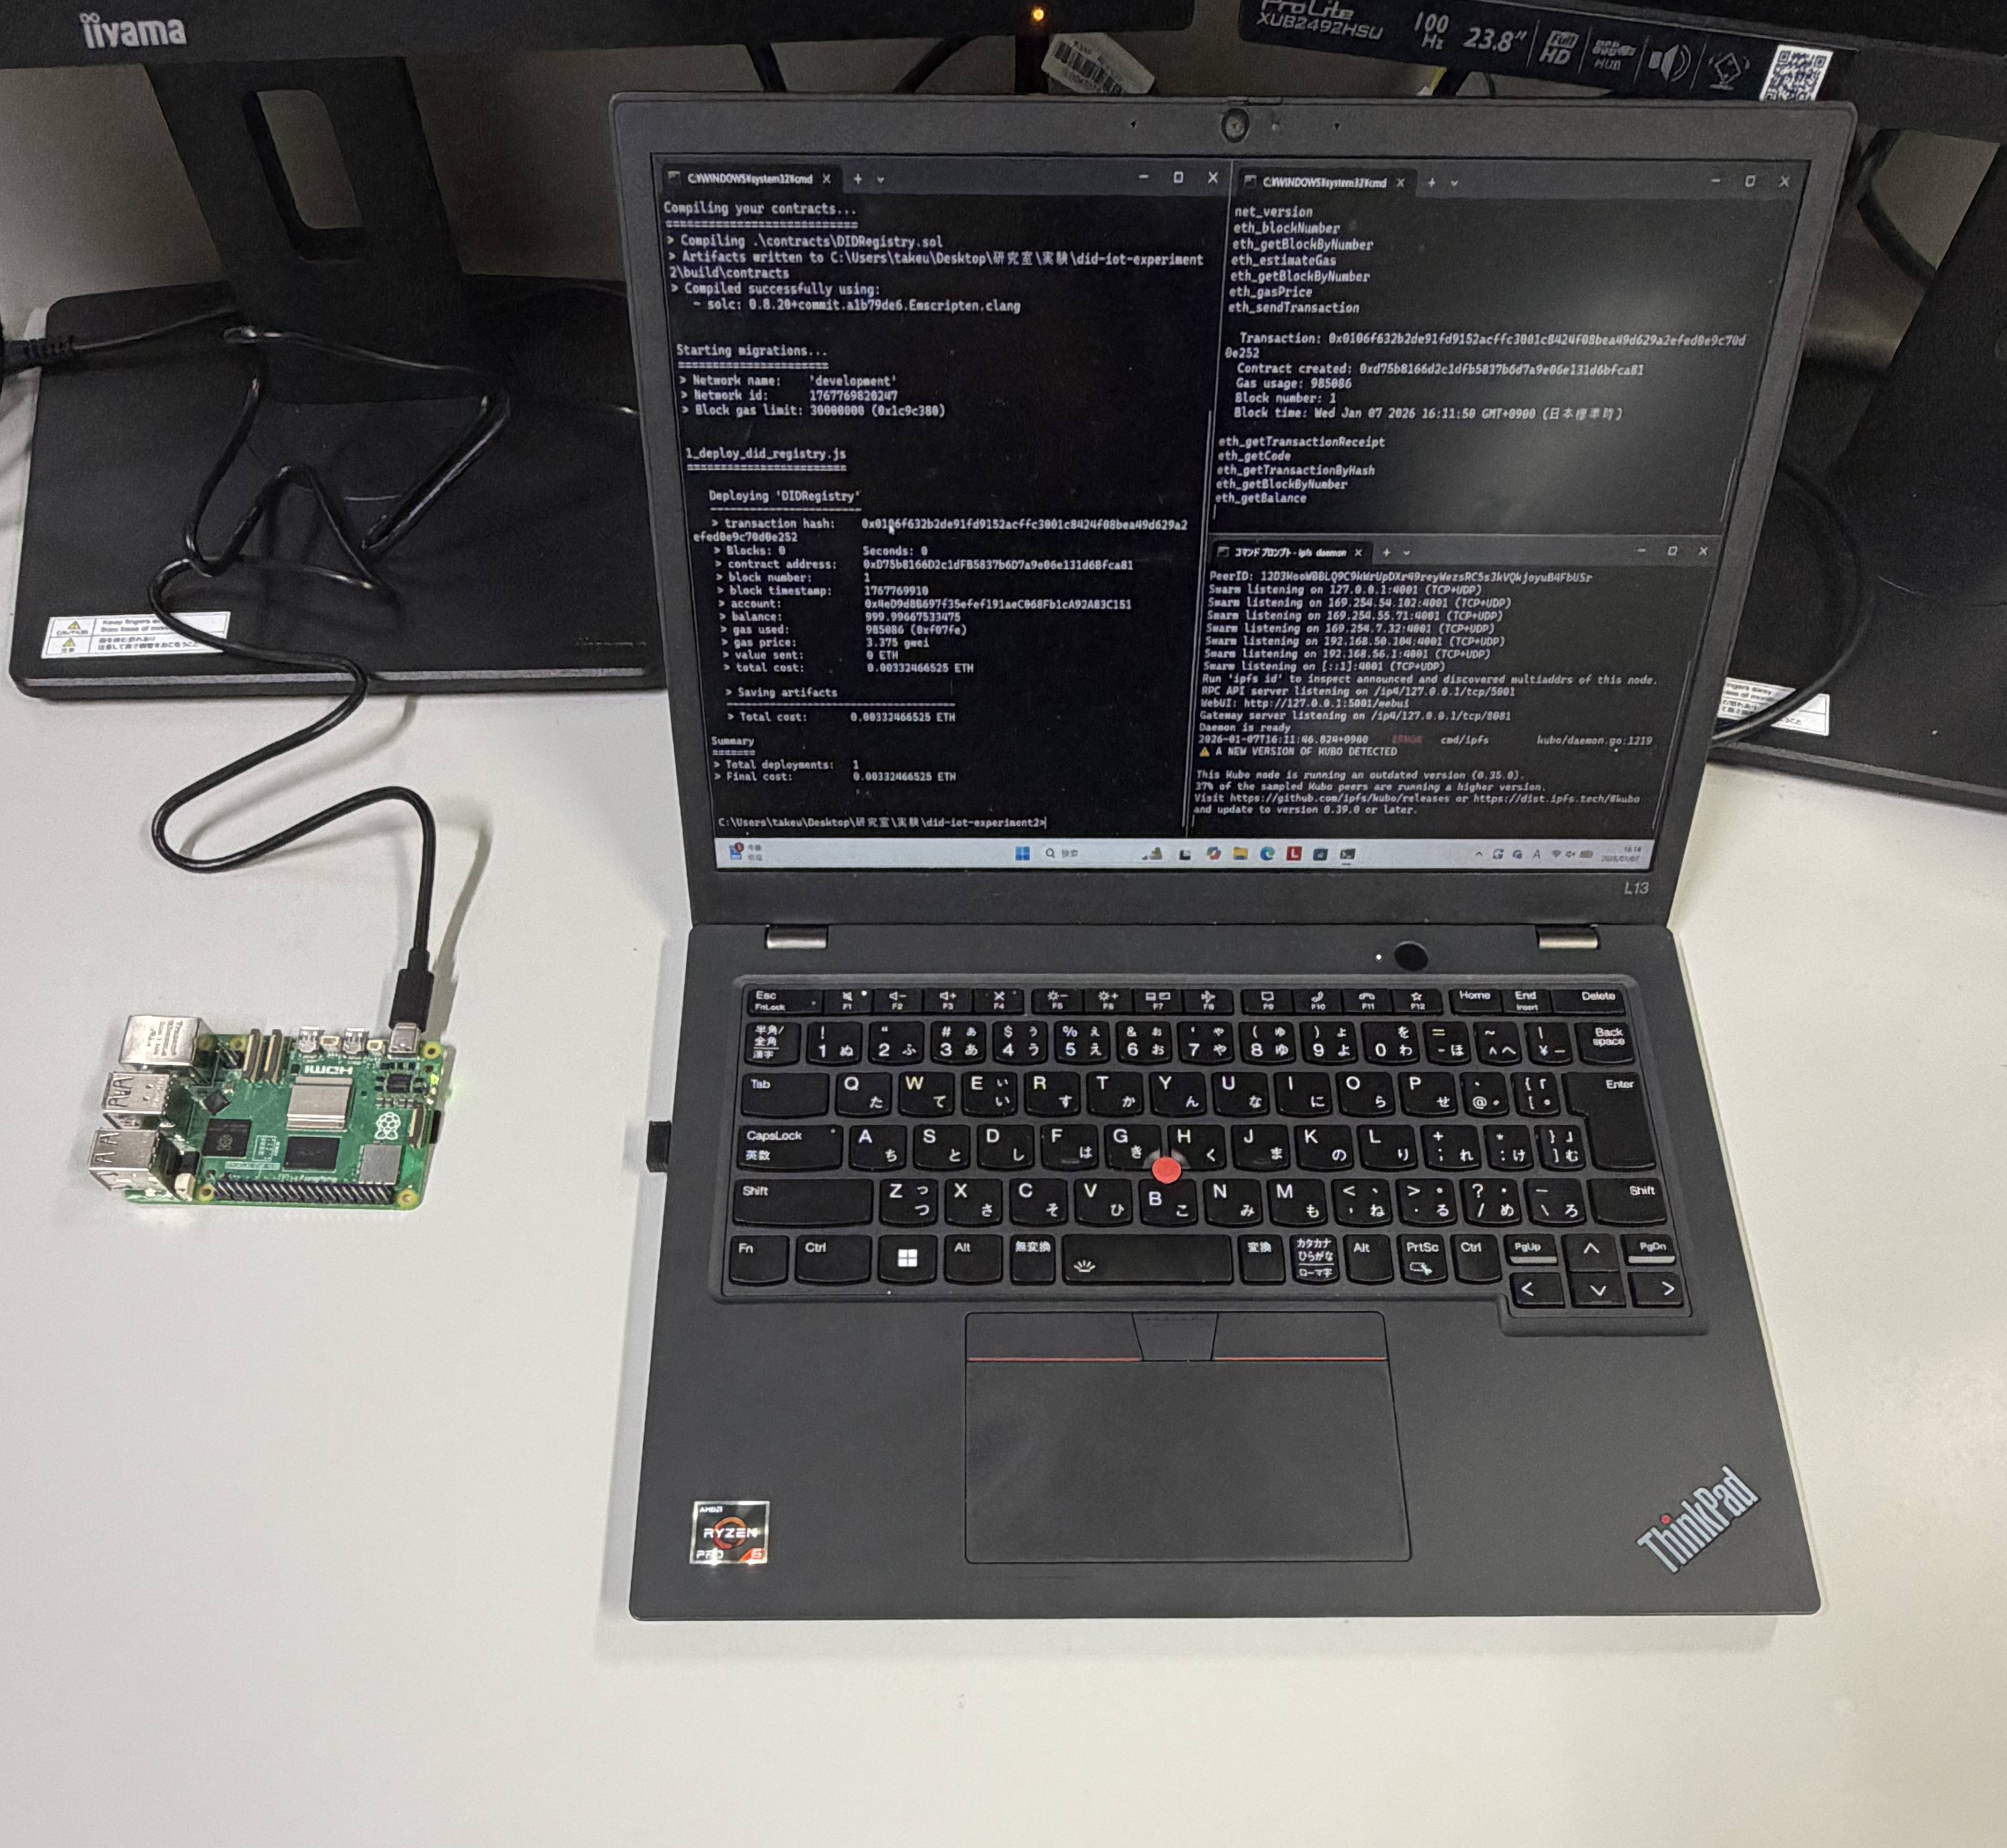
\includegraphics[width=0.7\linewidth]{figures/experiment_environment.png}
  \caption{実験環境の外観}
  \label{fig:experiment_photo}
\end{figure}

\begin{figure}[H]
  \centering
  \includegraphics[width=0.9\linewidth]{figures/experiment_environment_figure.png}
  \caption{実験環境の構成}
  \label{fig:experiment_structure}
\end{figure}

\subsection{実験方法}
本節では,本研究で構築したシステムに対して実施した実験方法を述べる.
実験は大きく次の2段階に分けて行った.

\begin{enumerate}
  \item \textbf{機能動作試験}
  
  DID Documentの登録,IoTデータのIPFSへの保存,CIDのブロックチェーンへの記録,発行者によるVC発行,検証者によるVC検証という一連の処理が正しく実行されることを確認した.

  \item \textbf{性能評価}
  
  提案システムにおける主要な処理について処理時間を計測し,
  VCの発行および検証処理に要する時間と他の処理時間を比較することで,
  DID/VCの導入がシステム全体の性能に与える影響,
  特に処理のボトルネックとなり得るかについて評価を行った.
  本評価における測定対象を以下に示す.

  \begin{itemize}
    \item IoTデータのIPFSアップロード時間
    \item ブロックチェーンへのCID登録時間
    \item VC発行処理時間
    \item VC検証処理時間
  \end{itemize}
\end{enumerate}

なお,本研究における「データ1件」とは,センサから取得された1時点分のIoTデータを表すJSONオブジェクト1つ分を指す.
具体的には,タイムスタンプ,温度,湿度,照度を含む以下の形式のJSONデータ1つを1件とする擬似データを使用している.

\begin{verbatim}
  {
    "timestamp": "2025-12-14 18:32:58",
    "temperature": 21.65,
    "humidity": 63.41,
    "light": 926
  }
\end{verbatim}

したがって,データ数10件,100件,1,000件とは,上記形式のJSONデータをそれぞれ10個,100個,1,000個まとめたファイルを対象として測定を行ったことを意味する.

\subsection{実験結果}

\subsubsection{機能動作試験の結果}
本研究で構築したシステムが,設計時に想定した一連の処理を正しく実行できるかを確認するため,
各処理を順に実行し,コマンドプロンプト上の出力結果をもとに機能動作試験を行った.

まず,図\ref{fig:register_did}に示すように,ユーザおよび発行者がそれぞれDIDを生成し,
対応するDID Documentを作成した後,スマートコントラクトを通じてブロックチェーンへ登録する処理を実行した.
出力結果から,DIDおよびDID Documentを正常が正常に生成され,トランザクションが成功していることを確認できる.

次に,図\ref{fig:ipfs_upload}に示すように,IoTデータをIPFSへアップロードする処理を実行した.
コマンドプロンプトには,アップロード対象ファイルに対応するCIDが表示されており,
データがIPFS上に正常に保存されたことが確認できる.

続いて,図\ref{fig:register_cid_to_bc}では,IPFS上に保存されたデータのCIDと,
そのデータの所有者を示すDIDをブロックチェーンへ記録する処理を示している.
出力結果から,CIDおよびDIDが対応付けられた形でスマートコントラクトに記録され,
処理が正常に完了していることが確認できる.

図\ref{fig:issue_vc}は,発行者がユーザに対してVCを発行する処理の実行結果を示している.
コマンドプロンプトには,VCの生成および発行処理が正常に完了した旨が出力されており,発行者によるVC発行が正しく行われたことが確認できる.

次に,図\ref{fig:sign_vc_by_userA}に示すように,ユーザAが発行されたVCに対して署名を行う処理を実行した.
出力結果から,ユーザAの秘密鍵を用いた署名処理が成功していることが確認でき,VCがユーザ本人によって承認された状態となっていることが分かる.

最後に,図\ref{fig:validate_vc}では,検証者がVCの検証処理を実行した結果を示している.
コマンドプロンプトの出力から,VCの署名検証およびDID Documentとの照合が成功し,
VCの正当性が確認されたことが分かる.

以上の結果より,DIDの生成・登録,IPFSへのデータ保存,CIDとDIDのブロックチェーン記録,
VCの発行・署名・検証という一連の処理が,提案システムにおいて問題なく実行できることを確認した.

\begin{figure}[H]
  \centering
  \includegraphics[width=0.95\linewidth]{figures/register_did.png}
  \caption{DIDおよびDID Documentの生成・登録処理の実行結果}
  \label{fig:register_did}
\end{figure}

\begin{figure}[H]
  \centering
  \includegraphics[width=0.95\linewidth]{figures/ipfs_upload.png}
  \caption{IPFSへのデータアップロードの実行結果}
  \label{fig:ipfs_upload}
\end{figure}

\begin{figure}[H]
  \centering
  \includegraphics[width=0.95\linewidth]{figures/register_cid_to_bc.png}
  \caption{CIDおよびDIDのブロックチェーンへの記録処理}
  \label{fig:register_cid_to_bc}
\end{figure}

\begin{figure}[H]
  \centering
  \includegraphics[width=0.95\linewidth]{figures/issue_vc.png}
  \caption{発行者がVCを発行する処理}
  \label{fig:issue_vc}
\end{figure}

\begin{figure}[H]
  \centering
  \includegraphics[width=0.95\linewidth]{figures/sign_vc_by_userA.png}
  \caption{UserAがVCに署名する処理}
  \label{fig:sign_vc_by_userA}
\end{figure}

\begin{figure}[H]
  \centering
  \includegraphics[width=0.95\linewidth]{figures/validate_vc.png}
  \caption{検証者がVCを検証する処理}
  \label{fig:validate_vc}
\end{figure}

\subsubsection{性能評価の結果}

本研究では,提案システムの実運用を想定した際に,DID/VCを統合したことが性能上のボトルネックとなり得るかを評価することを目的として,
各処理に要する時間の計測を行った.

性能測定は,各処理は20回繰り返し実行した際の平均処理時間を算出することで行った.
まず,IPFSへのIoTデータアップロード処理の性能を評価した.
その結果,データ数10件(931bytes)から1,000件(96,793bytes)までのいずれの場合においても,
平均処理時間は約19~21msで推移しており,データサイズの増加に対して大きな遅延は確認されなかった.
また,スループットはデータ数の増加に伴い向上しており,IPFSがIoTデータの集約保存に対して十分な性能を有することが確認できた.

次に,ブロックチェーンへのCID登録処理に要する時間を計測した.
本処理では,データ内容に依存しない条件下において,平均処理時間は63.60msであり,トランザクション処 理として一定の時間を要するものの,
安定した性能を示した.

これらの処理と比較し検討するため,VCの発行処理および検証処理に要する時間を計測した.


まず,VCの発行に要する時間を計測した結果,平均処理時間は10.45msであり,
IPFSアップロード処理およびブロックチェーンへの記録処理と比較しても短い処理時間であった.

一方,VCの検証処理に要する平均時間は155.78msであり他の処理と比較して相対的に長い処理時間を要する結果となった.

以上の性能評価結果を表\ref{tab:performance_results}にまとめる.

\begin{table}[h]
  \centering
  \caption{各処理における性能評価結果}
  \label{tab:performance_results}
  \begin{tabular}{l|l|r}
    \hline
    処理内容 & 条件 & 平均処理時間 \\ \hline
    IPFSアップロード & 10件(931bytes) & 19.11ms \\
    IPFSアップロード & 100件(9,279bytes) & 20.78ms \\
    IPFSアップロード & 1,000件(96,793bytes) & 21.20ms \\
    ブロックチェーン登録 & --- & 63.60ms \\
    VC発行 & --- & 10.45ms \\
    VC検証 & --- & 155.78ms \\
    \hline
  \end{tabular}
\end{table}


\subsection{考察}
本章では,前章で示した実験結果を踏まえ,提案システムにおいてDIDおよびVCを統合したことがシステム全体の性能に与える影響について考察する.

\subsubsection{DID/VCが性能に与える影響}
まず,VCの発行処理に着目する.
性能評価の結果より,IPFSへのIoTデータアップロード時間は約19~21msで推移し,ブロックチェーンへのCID記録処理は平均63.60msを要することが確認されている.
これらの処理と比較すると,VCの発行処理に要する平均時間は10.45msと短く,システム全体の処理性能に与える影響は小さい.
このことから,VCの発行処理が提案システムの動作において性能上のボトルネックとなる可能性は低いと考えられる.

次に,VCの検証処理に着目する.
VCの検証にかかる処理は155.78msであり,IPFSへのアップロード処理やブロックチェーンへのCID記録処理と比較して,
相対的に長い処理時間を要する結果となった.

しかしながら,VCの検証処理は,IoTデータの保存や更新といった高頻度に実行される処理とは異なりデータの取引時といった特定のタイミングでの実行を想定している.
そのため,通常の運用形態においてはシステム全体の性能に与える影響は限定的であると考えられる一方,
検証処理の実行頻度が高くなる場合には,性能上のボトルネックとなる可能性も否定できない.

\subsubsection{今後の課題}
本稿で提案したシステムは,特定の中央集権的管理主体に依存せず,分散的にIoTデータを管理することを目的として設計した.

しかしながら,ユーザが保有するIoTデータの正当性を保証する手段としてVCを用いる場合,
その発行主体として企業などの特定の組織に依存せざるを得ない.
この点において,提案システムは一部に中央集権的な管理構造を内包しているといえる.

したがって,完全に分散化されたデータ管理システムの実現という観点からは,
データの正当性保証を特定の組織に依存せずに実現する仕組みについて,
今後さらなる検討が必要である.

また,IPFSはコンテンツアドレス型の分散ストレージであり,
CIDを知る第三者が当該データを取得可能であるという特性を有する.
そのため,CIDが第三者に漏洩した場合においてもデータの内容が不正に閲覧されないよう,
データの暗号化などによって機密性を確保する仕組みを併せて検討する必要がある.

\section{まとめ}
本研究では,IoT機器の増加に伴い顕在化するデータ管理のスケーラビリティ,セキュリティ,
およびプライバシー保護といった課題に対し,ユーザ主権型IDに基づく分散型IoTデータ管理システムを提案した.
提案システムは,IPFS,ブロックチェーン,DID/VCを連携させることで,
中央集権的管理主体に依存せずにIoTデータの管理と真正性検証を可能とすることを目的として設計した.

本研究では,まずIPSFを用いてIoTデータ本体を分散的に保存し,得られたCIDをブロックチェーン上に記録することで,
データの改ざん耐性と参照可能性を確保した.
さらに,DIDおよびDID Documentを導入することで,
分散環境においてもデータ保有者の識別と公開鍵の正当性を検証可能とした.
加えて,発行者がVCを発行し,ユーザ自身も署名を付与する仕組みを構築することで,
IoTデータが正当なデバイスによって生成されたものであることと,
ユーザが当該データの正当な保有者であることを第三者が検証できる構成を実現した.

提案システムに対して字視した機能動作試験の結果,
DIDの生成・登録,IoTデータのIPFSへの保存,CIDとDIDのブロックチェーンへの記録,
VCの発行・署名・検証という一連の処理が,想定通り正しく実行されることを確認した.
これにより,IPFS,ブロックチェーン,DID/VCを統合した分散型データ管理基盤が,
データとその保有者の正当性を一貫して保証できることを示した.

また,性能評価を通じて,各処理に要する時間を計測した結果,
VCの発行処理はIPFSへのアップロード処理やブロックチェーンへのCID記録処理と比較して短時間で完了し,
システム全体の性能に与える影響は小さいことが確認された.
一方,VCの検証処理は他の処理と比較して相対的に長い処理時間を要する結果となったが,
本研究で想定する運用形態では高頻度に実行される処理ではないため,
通常の利用においては性能上のボトルネックとなる可能性は限定的であると考えられる.

以上より,本研究は,DID/VCを用いることで,IoTデータの真正性と保有者の正当性を分散的に検証可能な管理体制を構築できることを示し,
その実装可能性および性能特性を明らかにした点に意義がある.
今後の課題として,VCの発行主体を特定の組織に依存しない正当性保証の仕組みの検討や,
CIDの漏洩時にもデータの機密性を確保するための暗号化手法の導入が挙げられる.

\bibliographystyle{junsrt}
\bibliography{references}
\end{document}
